\documentclass[10pt,a4paper]{scrartcl}
\usepackage[utf8]{inputenc}
\usepackage[german]{babel}
\usepackage[T1]{fontenc}
\usepackage{amsmath}
\usepackage{amsfonts}
\usepackage{amssymb}
\usepackage{graphicx}
\usepackage{float}
\usepackage{booktabs}
\begin{document}
\title{Bedienungsanleitung}
\author{Clemens Büsch, Dennis Ernst}
\date{}
\subtitle{Optische Übertragungsstrecke Hochspannungslabor}
\maketitle
\tableofcontents

\newpage
\section{Übersicht}
Die Optische Übertragungstrecke für das Hochspannungslabor besteht aus zwei Einheiten, welche jeweils für das Senden und für das Empfangen des Messsignals(AC gekoppelt) zuständig sind.  \\ \\ 
\begin{center}
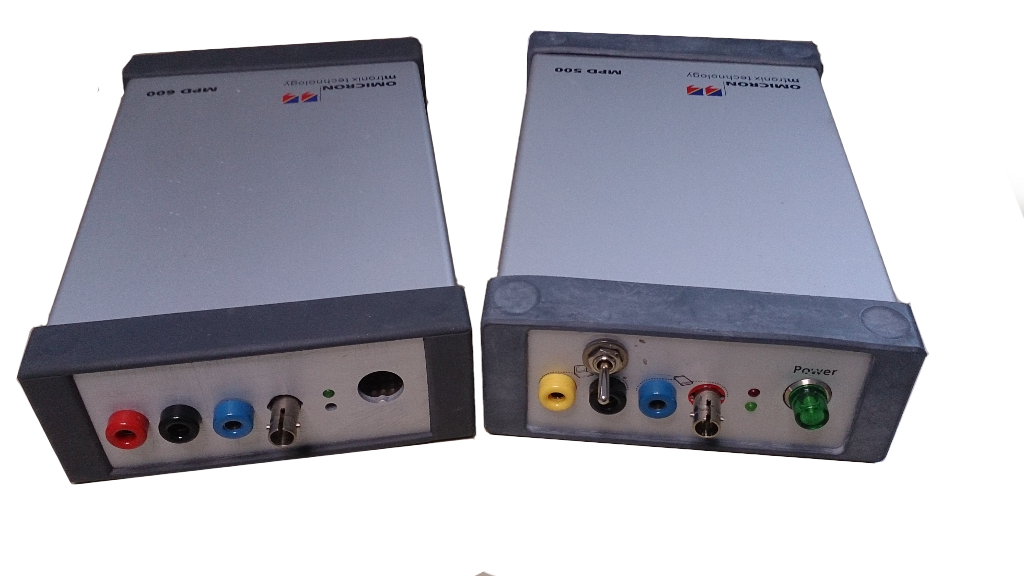
\includegraphics[scale=0.4]{gfx/title.JPG}
\end{center}


\section{Technische Spezifikation}
\begin{table}[h!]
\centering 
\begin{tabular}{@{} lr @{}}
 \toprule
 \textbf{Gesamtsystem:} \\
 Bandbreite & $10-100 Hz$ \\
  \midrule
  \textbf{Sendeeinheit:} \\
  Betriebsspannung & $\pm 12V$ \\
  Impedanz & $12k\Omega$ / $22k\Omega$   \\
  Maximale Eingangsamplitude & $6 V$\\
  \midrule
  \textbf{Empfangseinheit:}\\
  Betriebsspannung & $\pm 5V$ \\
  Maximale Ausgangsamplitude &$ 5V$\\
  
 \bottomrule
\end{tabular}

\end{table}
\newpage

\section{Anschluss Sendeeinheit}
\subsection{Schnittstellen Vorderseite}
\begin{figure}[H]
\begin{minipage}[t]{6cm}
\vspace{0pt}

\begin{enumerate}
\item Buchse +12V
\item Buchse GND
\item Buchse -12V
\item Buchse Laserdiode \\(Lichtwellenleiter)
\item Signalleuchte Impedanz 12 $k\Omega$
\item Betriebsleuchte
\item Signalleuchte Impedanz 22 $k\Omega$
\item Ein/Aus Schalter 
\end{enumerate}
\end{minipage}
\hfill
\begin{minipage}[t]{6.5cm}
\vspace{0pt}
\centering
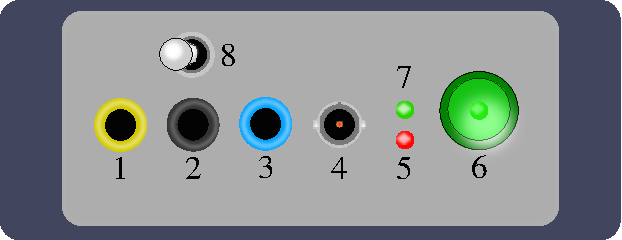
\includegraphics[scale=0.7]{gfx/tx-front.pdf}
\caption{Vorderseite Sendeeinheit}
\label{fig:tx-front}
\end{minipage}
\end{figure}

\subsection{Schnittstellen Rückseite}
\begin{figure}[H]
\begin{minipage}[t]{6cm}
\vspace{0pt}
\centering
\begin{enumerate}
\setcounter{enumi}{8}
\item Impedanzschalter
\item BNC-Buchse Eingangssignal
\end{enumerate}
\end{minipage}
\hfill
\begin{minipage}[t]{6.5cm}
\vspace{0pt}
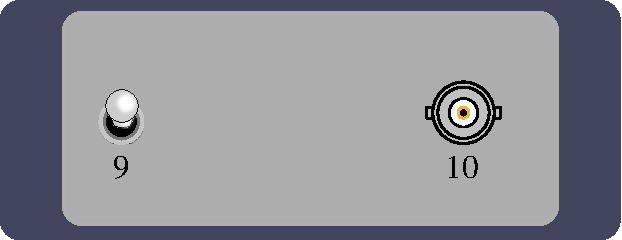
\includegraphics[scale=0.7]{gfx/tx-back.pdf}
\caption{Rückseite Sendeeinheit}
\label{fig:tx-back}
\end{minipage}
\end{figure}

\subsection{Inbetriebnahme Sendeeinheit}
\begin{itemize}
\item Bevor die Sendeeinheit mit anderen Komponenten verbunden wird muss diese ausgeschaltet sein. Hierzu muss Schalter(8) in linker Position sein.
\item Danach gilt es die Versorgungsspannung zu verbinden. Dabei ist zu beachten die beigelegte V-Verbindung mit den jeweiligen Akkus zu verwenden.
\item Beim Aufbau ist besonders auf die jeweiligen Kabel- und Buchsenfarben(1,2,3) zu achten! \textbf{Achtung ein falscher Anschluss(Verpolung) kann zur Zerstörung des Gerätes führen!}
\item Anschließend wird die vom Messobjekt kommende Leitung an die BNC-Buchse(10) angekoppelt.
\item Sobald die Sendeeinheit einen festen Platz hat, kann der Lichtwellenleiter mit der Laserdiode(4) verbunden werden. Hierbei gilt es zu beachten, dass der Lichtwellenleiter nicht zu großer mechanischer Belastung ausgesetzt wird.
\item Nun kann die Sendeeinheit eingeschaltet werden in dem der Schalter(8) in rechte Position gebracht wird.
\item Schlussendlich wird die gewünschte Impedanz über den Schalter(9) eingestellt. Die eingestellte Impedanz wird über die Signalleuchten(5,7) angegeben.
\end{itemize}

Die Sendeeinheit ist nun betriebsbereit. 


\section{Anschluss Empfangseinheit}
\subsection{Schnittstellen Vorderseite}
\begin{figure}[H]
\begin{minipage}[t]{6cm}
\vspace{0pt}
\begin{enumerate}
\item Buchse +5V
\item Buchse GND
\item Buchse -5V
\item Empfangsdiode Lichtwellenleiter
\item Signalleuchte (Signal vorhanden)
\end{enumerate}
\centering
\end{minipage}
\hfill
\begin{minipage}[t]{6.5cm}
\vspace{0pt}
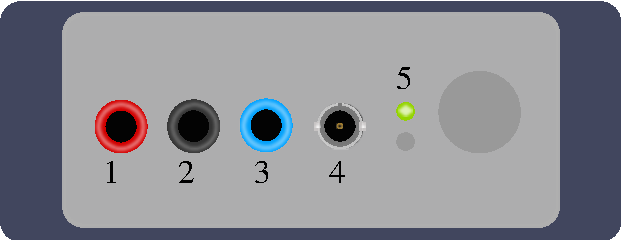
\includegraphics[scale=0.7]{gfx/rx-front.pdf}
\caption{Vorderseite Empfangseinheit}
\label{fig:Bild3}
\end{minipage}
\end{figure}

\subsection{Schnittstellen Rückseite}
\begin{figure}[H]
\begin{minipage}[t]{6cm}
\vspace{0pt}
\begin{enumerate}
\setcounter{enumi}{5}
\item BNC-Buchse Ausgangssignal
\end{enumerate}
\end{minipage}
\hfill
\begin{minipage}[t]{6.5cm}
\vspace{0pt}

\includegraphics[scale=0.7]{gfx/rx-back.pdf}
\caption{Rückseite Empfangseinheit}
\label{fig:Bild4}
\end{minipage}
\end{figure}

\subsection{Inbetriebnahme Empfangseinheit}
Die Sendeeinheit wird mit einem Labornetzteil betrieben. Dieses ist bei Verkabelung aus.
Die Versorgungsspannung wird an die Buchsen(1,2,3) angeschlossen. \textbf{Achtung ein falscher Anschluss(Verpolung) kann zur Zerstörung des Gerätes führen!}. Anschließend wird die zum Messgerät führende BNC-Kupplung an die BNC-Buchse(6) angeschlossen. Sobald die Empfangseineinheit einen festen Platz hat wird der Lichtwellenleiter mit der Empfangsdiode(4) verbunden. Hierbei gilt es zu beachten, dass der Lichtwellenleiter nicht zu großer mechanischer Belastung ausgesetzt wird. Anschließend wird das Gerät in Betrieb genommen indem das Labornetzteil eingeschaltet wird. Wenn alles korrekt verbunden ist und ein Signal anliegt leuchtet die Signalleuchte(6).
Die Empfangseinheit ist nun Betriebsbereit und die Messung kann beginnen.
\end{document}